%%%%%%%%%%%%%%%%%%%%%%%%%%%%%%%%%%%% Chapter Template

\chapter{Stability} 	% Main chapter title
\label{Chapter3} 		% For referencing the chapter elsewhere, usage \ref{Chapter1}

%%%%%%%%%%%%%%%%%%%%%%%%%%%%%%%%%%%%

During discussions with the team riders testing the new prototypes, it became evident that another critical phenomenon significantly impacted kite performance. 

In general, when a rider is moving downwind, they prefer the kite to exhibit a strong forward impulse, causing it to move deep into the wind window, even if the athlete maintains bar tension. Conversely, when a rider is heading upwind, the kite naturally wants to surge forward, especially when it flies at high Reynolds numbers and low angles of attack. But in contrast to downwind conditions, when the kite surges forward while going upwind, it tends to move out of the wind window. When the brakes halt the kite's forward movement after "shooting" forward, if the kite continues to progress forward due to a negative pitching moment, it may collapse. 

The manner in which a kite behaves when coming to a stop after moving forward, and how it attains its moment equilibrium, is frequently referred to as \textbf{"stability"} in kitesurfing. An unstable kite is one that continues to move forward even after the brakes have stopped it during a "shoot" (dynamic forward flight); it is a kite that proves challenging, and at times impossible, to control because it \textbf{collapses}.







\begin{figure}[H]
    \centering
    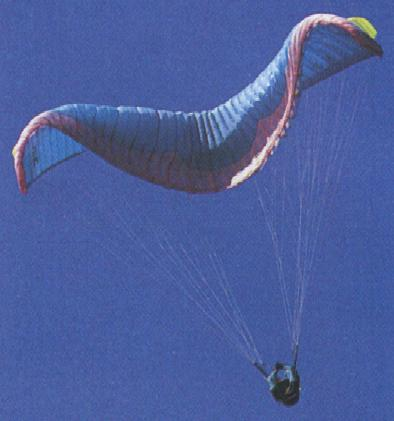
\includegraphics[width = 0.5\linewidth]{figures/Stability/front collapse.jpg}
    \caption{Picture of a paraglider pilot experiencing a front collapse}
    \label{fig:Picture of a paraglider pilot experiencing a front collapse}
\end{figure}


%%%%%%%%%%%%%%%%%%%%%%%%%%%%%%%%%%%%%%%%%%%%%%%%%%%%%%%%%%%%%%%%%%%%%%%%%%%%%%%%
%%%%%%%%%%%%%%%%%%%%%%%%%%%%%%%%%%%% SECTION 1 %%%%%%%%%%%%%%%%%%%%%%%%%%%%%%%%%
%%%%%%%%%%%%%%%%%%%%%%%%%%%%%%%%%%%%%%%%%%%%%%%%%%%%%%%%%%%%%%%%%%%%%%%%%%%%%%%%

\section{The aerodynamic definition of stability}
\label{sec:Ch3.1}

This issue of stability is well known in the paragliding world. As the physics is quite the same and the stakes are much higher, the Ozone paragliders designers have been able to help me translating the notion of stability in terms of aerodynamics. 

Contrary to the popular belief, a kite doesn't collapse when its incidence becomes negative, but before. "the collapse comes from the fact that the A lines bend more than the B lines under their own aerodynamic drag", according to the Ozone paraglider designers. \\

\begin{wrapfigure}{r}{0.5\textwidth}
\centering
    \includegraphics[width=0.4\textwidth]{figures/Stability/Schéma AB.png}
    \caption{A lines, B lines and lift on a kite airfoil}
    \label{fig:A lines, B lines and lift on an airfoil}
\end{wrapfigure}
Assuming that A lines drag and B lines drag are the same, for the kite to be stable, the tension in the A lines must be higher than the tension in the B lines. It also means that the aerodynamic force component collinear with the lines must be higher in the A lines than the B lines.\\

% \vspace{0.5cm}
Assuming that A lines and B lines are parallels near their towpoints (where the kite lines are tied) and considering a LIFT that represents the aerodynamic force component collinear with the lines, we have : 

\begin{figure}[H]
\centering
    \includegraphics[width=0.9\textwidth]{figures/Stability/schéma tension AB.png}
    \caption{A and B tensions on a kite airfoil}
    \label{fig:A and B tensions on a kite airfoil}
\end{figure}

\begin{equation}
\left \{
    \begin{array}{r c l}
        T_{A} = LIFT \frac{X_{B} - X_{cp}}{X_{B} - X_{A}} \\
        T_{B} = LIFT \frac{X_{cp} - X_{A}}{X_{B} - X_{A}} 
    \end{array}
    \right .
   \label{tension AB}
\end{equation}

\begin{equation}
    T_{A} \geq T_{B}M_{S} \iff X_{cp} \leq  \frac{X_{B}+X_{A}}{2M_{S}}
    \label{eq:last equation}
\end{equation}

With $M_{S}$ the static margin.

\textbf{As a result, we understand here that the aerodynamic force position along the chord Xcp is a measure of the kite stability}.\\


%%%%%%%%%%%%%%%%%%%%%%%%%%%%%%%%%%%%%%%%%%%%%%%%%%%%%%%%%%%%%%%%%%%%%%%%%%%%%%%%
%%%%%%%%%%%%%%%%%%%%%%%%%%%%%%%%%%%% SECTION 3 %%%%%%%%%%%%%%%%%%%%%%%%%%%%%%%%%
%%%%%%%%%%%%%%%%%%%%%%%%%%%%%%%%%%%%%%%%%%%%%%%%%%%%%%%%%%%%%%%%%%%%%%%%%%%%%%%%

\section{The theoretical existing kite stability}
\label{sec:Ch3.2}

To corroborate the aerodynamic concept of stability as outlined in section \ref{sec:Ch3.1}, a stability graph denoted as $X_{cp}(C_{L})$ was generated for each kite subjected to testing by our team riders. \\

It is known that : 
\begin{itemize}
    \item The R1 V4 is a very stable kite
    \item The R1 V5 is more stable than the VMG ( but less performant ) 
    \item The Vmg is close to the limit of stability
    \item The R1 V5 Satori3 is more unstable than the VMG but still stable ( if well trimmed )
    \item "Limit stability" refers to an airfoil that has undergone testing by Ozone paraglider team pilots and is regarded as the threshold of stability. In this context, it serves as an initial reference.
\end{itemize}

Running 2D simulations on these kites airfoils with aerosandbox, the following results have been obtained at 18knots and angles of attack from 2° to 13° : 

\begin{figure}[H]
    \centering
    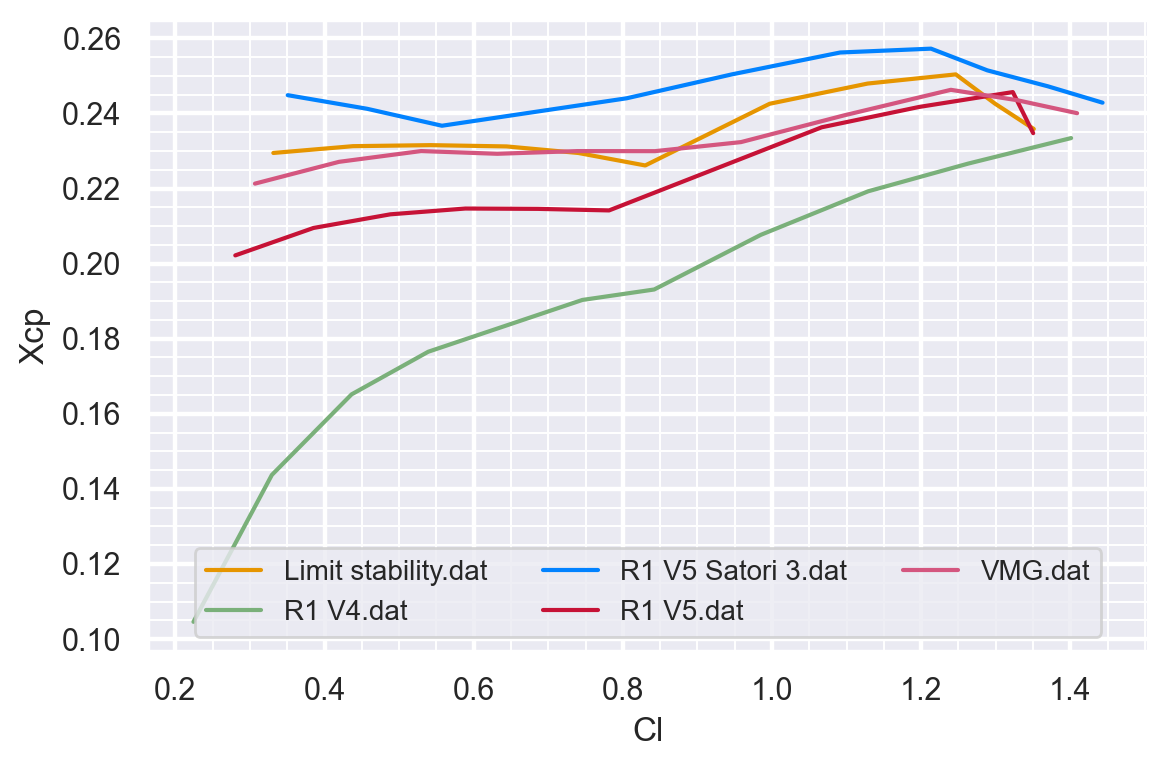
\includegraphics[width=1.0\textwidth]{figures/Stability/airfoils stability.png}
    \caption{$X_{Cp}$ plot against $C_{L}$ }
    \label{fig:X_{Cp} plot against C_{L}}
\end{figure}

It's worth noting that since stability is already noticeable on the beach, when the athlete's speed is at 0 knots, the value of 18 knots (wind speed) serves as a suitable benchmark for comparison with the feedback from the team riders. This is particularly pertinent because when they are stationary on the beach, there are fewer external factors that could affect the results compared to when they are actively riding out at sea.

The figure \ref{fig:X_{Cp} plot against C_{L}} shows that the aerodynamic definition of a kite stability established in \ref{sec:Ch3.1} is in line with the pro kitesurfers' feelings. 

Moreover, the figure \ref{fig:X_{Cp} plot against C_{L}} shows two characteristics that seem to be sources of instability : 
\begin{itemize}
    \item \textbf{high Xcp values}
    \item \textbf{A negative slope of the Xcp curve at low angles of attack}
\end{itemize}

Furthermore, it can be deduced from equation \ref{eq:last equation}, taking into account that for the present kites $X_{A} = 0.07$ and $X_{B} = 0.63$, and considering that $X_{cp} = 0.26$ serves as the stability threshold as depicted in figure \ref{fig:X_{Cp} plot against C_{L}}: \\

\underline{$M_{S} = 1.35$}

%%%%%%%%%%%%%%%%%%%%%%%%%%%%%%%%%%%%%%%%%%%%%%%%%%%%%%%%%%%%%%%%%%%%%%%%%%%%%%%%
%%%%%%%%%%%%%%%%%%%%%%%%%%%%%%%%%%%% SECTION 3 %%%%%%%%%%%%%%%%%%%%%%%%%%%%%%%%%
%%%%%%%%%%%%%%%%%%%%%%%%%%%%%%%%%%%%%%%%%%%%%%%%%%%%%%%%%%%%%%%%%%%%%%%%%%%%%%%%

\section{The add of stability in the airfoil optimization}
\label{sec:Ch3.3}

Taking the stability matter into account, the next step was to generate an optimized airfoil, like in \ref{sec:Ch2.2}, with the add of a stability constraint in the algorithm. 

It is assumed that the more the airfoil is optimized, the more instable it becomes. This is something we can observe on the prototypes we test but also regarding of the figure \ref{fig:X_{Cp} plot against C_{L}}. 

Furthermore, figure \ref{fig:Stability comparison between the existing airfoils and the optimized one} illustrates that the presently optimized airfoil, discussed in Section \ref{sec:Ch2.2}, exhibited excessive instability, making it unsuitable for use in the upcoming prototype.

\begin{figure}[H]
    \centering
    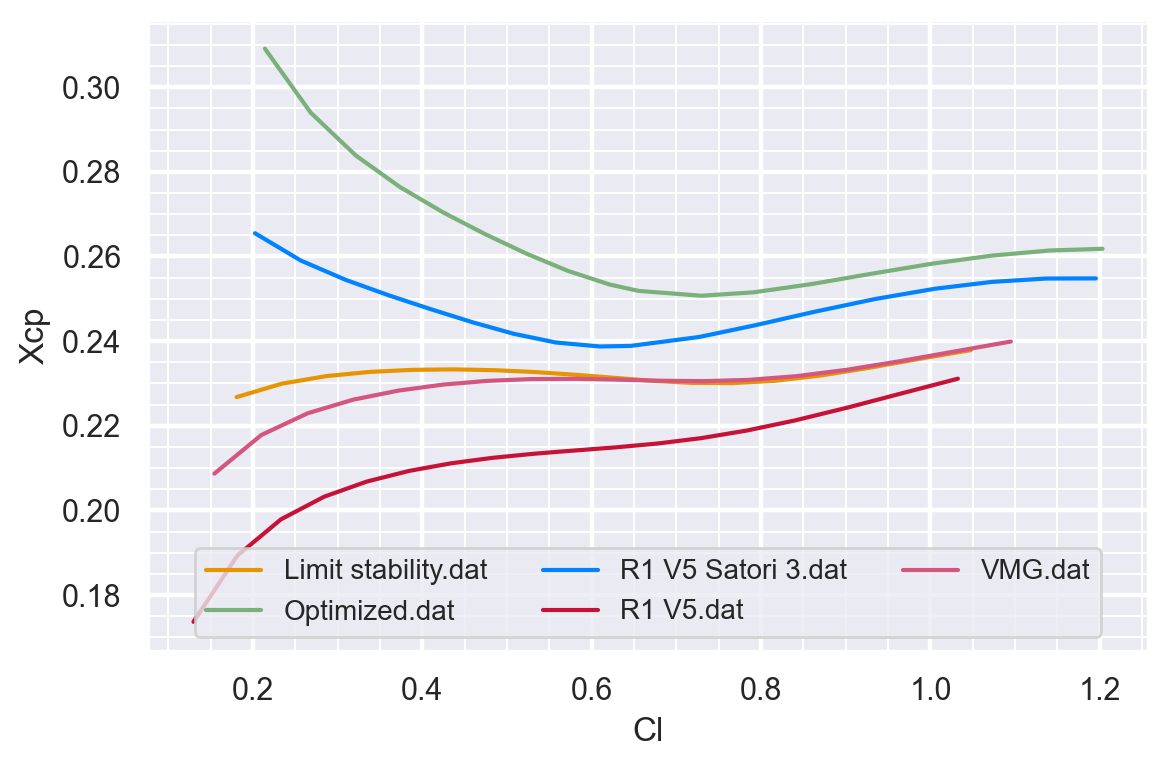
\includegraphics[width=1.0\textwidth]{figures/Stability/optimized airfoil stability.png}
    \caption{Stability comparison between the existing airfoils and the optimized one}
    \label{fig:Stability comparison between the existing airfoils and the optimized one}
\end{figure}

Consequently, the optimization algorithm was adapted to seek an airfoil that lies on the brink of instability while delivering the best possible performance, specifically by maximizing its finesse.

Nonetheless, the Ozone design team opted to delay the adjustment of the value of $M_{S}$, referenced in Section \ref{sec:Ch3.2}, until the team riders had the opportunity to test the optimized airfoil identified in Section \ref{sec:Ch2.2}. Given that the stability constraint imposes significant limitations on the optimization algorithm, it was prudent to first confirm that the current optimized airfoil exhibited instability. However, the team riders have not yet conducted tests on the optimized profile, and the value of $M_{S}$ remains to be verified.

Furthermore, this phase in airfoil design underscored the significance of the initial guess airfoil in the optimization process. It became evident that the algorithm encountered difficulties in reversing the stability graph of an airfoil. In fact, the sign of the slope in the $X_{cp}$ plot at low Cl values would remain unaltered during the optimization process. This implies that starting with an unstable airfoil as the initial guess would not lead to a stable optimized airfoil.